\begin{figure}[H]
\centering

\begin{subfigure}{.33\textwidth}
  \centering
  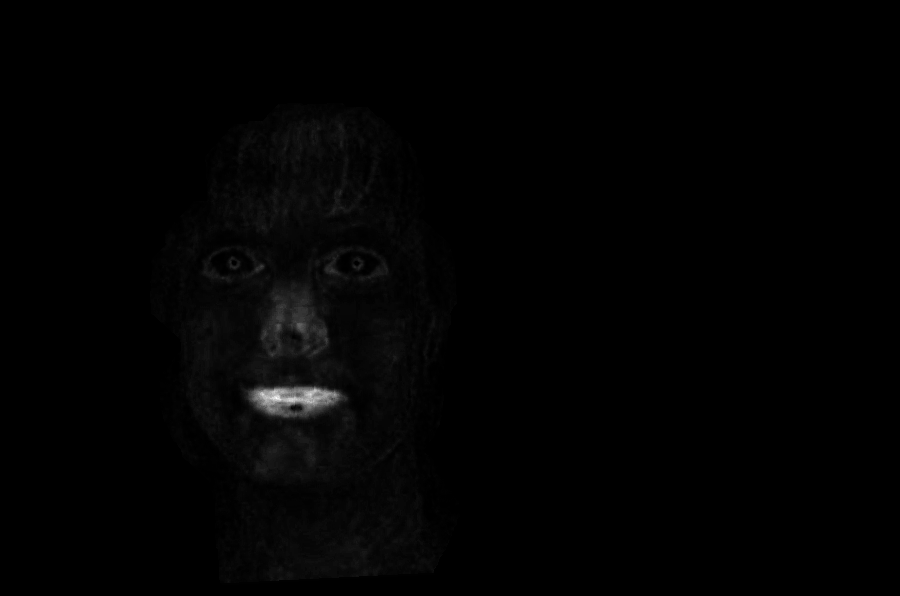
\includegraphics[width=0.95\textwidth]{img/fd/MouthMask.png}
  \caption{}
  % \label{fig:sub1}
\end{subfigure}%
\begin{subfigure}{.33\textwidth}
  \centering
  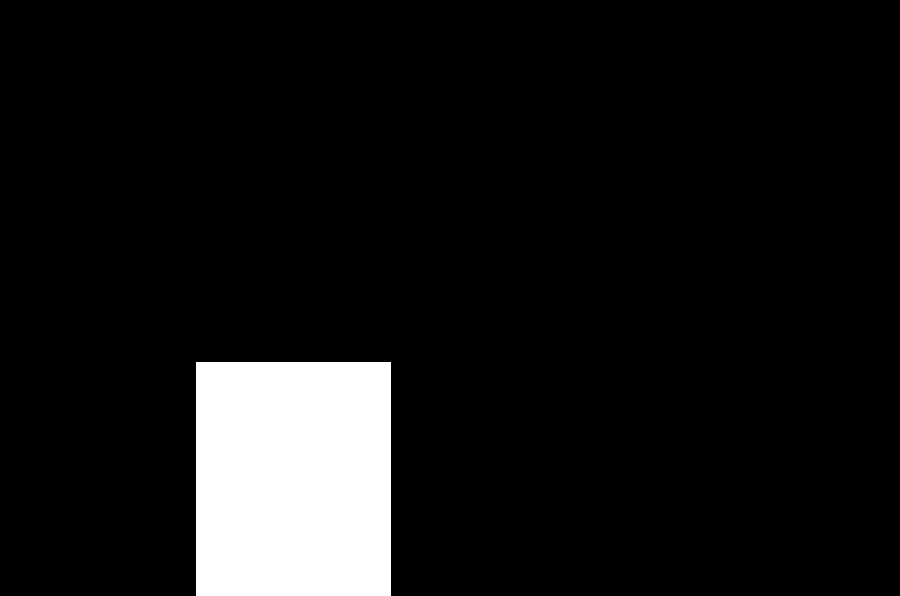
\includegraphics[width=0.95\textwidth]{img/fd/notNonMouthMask.png}
  \caption{}
  % \label{fig:sub1}
\end{subfigure}%
\begin{subfigure}{.33\textwidth}
  \centering
  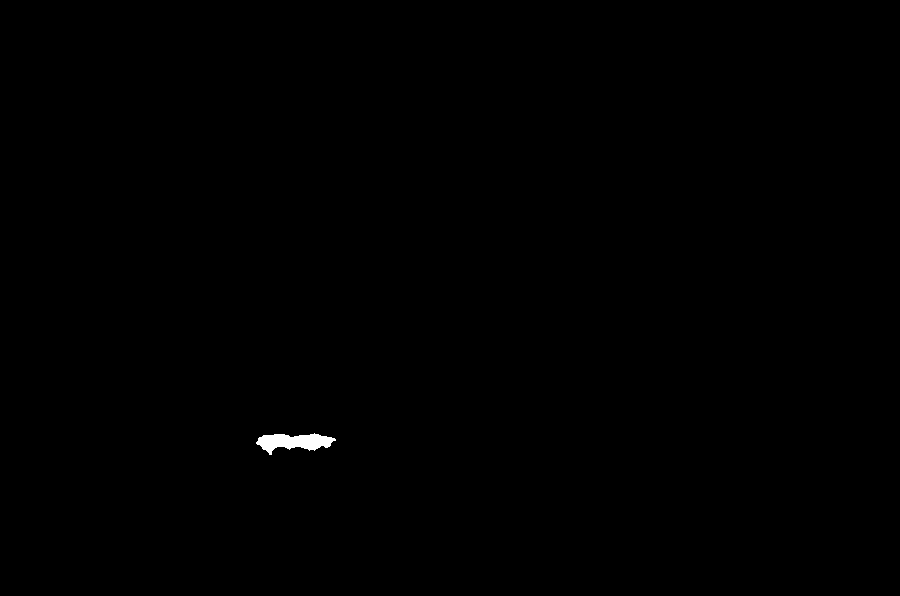
\includegraphics[width=0.95\textwidth]{img/fd/MouthBlob.png}
  \caption{}
  % \label{fig:sub1}
\end{subfigure}%

\caption{Process of computing the location of the mouth. (a) show the mouth map, (b) a mask for the region where the mouth should be located while (c) show the final mouth mask.}
\label{fig:mouthMap}
\end{figure}